\documentclass[11pt]{article}
\usepackage{amsmath}
\usepackage{amssymb}
\usepackage{graphicx}
\usepackage{tabularx}
\usepackage{fancyhdr}
\usepackage{lastpage}

% Page layout
\usepackage[top=1in, bottom=1in, left=1in, right=1in]{geometry}

% Header and footer
\pagestyle{fancy}
\fancyhf{}
\rfoot{Page \thepage}
\renewcommand{\headrulewidth}{0pt}

% Modified Question command with left-aligned number
\newcommand{\questiona}[2]{
    \noindent\textbf{Q#2.} #1 \hfill \textbf{[1 Mark]}
}

\newcommand{\questionb}[2]{
    \noindent\textbf{Q#2.} #1 \hfill \textbf{[2 Marks]}
}

\begin{document}

% Title section with horizontal line
\begin{center}
    \Large\textbf{GATE 2017 - Electronics and Communication Engineering (ECE)} \\
    \large\textbf{General Aptitude and Technical Questions} \\
    \rule{\textwidth}{0.5pt} % Horizontal line below heading
\end{center}

\vspace{0.5cm}

% General Aptitude Section
\section*{General Aptitude}

\questiona{The ninth and the tenth of this month are Monday and Tuesday \_\_\_\_\_.}{1}
\begin{enumerate}
    \item[(A)] figuratively  
    \item[(B)] retrospectively  
    \item[(C)] respectively  
    \item[(D)] rightfully  
\end{enumerate}

\vspace{0.5cm}

\questiona{It is \_\_\_\_\_ to read this year's textbook \_\_\_\_\_ the last year's.}{2}
\begin{enumerate}
    \item[(A)] easier, than  
    \item[(B)] most easy, than  
    \item[(C)] easier, from  
    \item[(D)] easiest, from  
\end{enumerate}

\vspace{0.5cm}

\questiona{A rule states that in order to drink beer, one must be over 18 years old. In a bar, there are 4 people. P is 16 years old, Q is 25 years old, R is drinking milkshake and S is drinking a beer. What must be checked to ensure that the rule is being followed?}{3}
\begin{enumerate}
    \item[(A)] Only P's drink  
    \item[(B)] Only P's drink and S's age  
    \item[(C)] Only S's age  
    \item[(D)] Only P's drink, Q's drink and S's age  
\end{enumerate}

\vspace{0.5cm}

\questiona{Fatima starts from point P, goes North for 3 km, and then East for 4 km to reach point Q. She then turns to face point P and goes 15 km in that direction. She then goes North for 6 km. How far is she from point P, and in which direction should she go to reach point P?}{4}
\begin{enumerate}
    \item[(A)] 8 km, East  
    \item[(B)] 12 km, North  
    \item[(C)] 6 km, East  
    \item[(D)] 10 km, North  
\end{enumerate}

\vspace{0.5cm}

\questiona{500 students are taking one or more courses out of Chemistry, Physics, and Mathematics. Registration records indicate course enrolment as follows: Chemistry (329), Physics (186), Mathematics (295), Chemistry and Physics (83), Chemistry and Mathematics (217), and Physics and Mathematics (63). How many students are taking all 3 subjects?}{5}
\begin{enumerate}
    \item[(A)] 37  
    \item[(B)] 43  
    \item[(C)] 47  
    \item[(D)] 53  
\end{enumerate}

\vspace{0.5cm}

\questionb{"If you are looking for a history of India, or for an account of the rise and fall of the British Raj, or for the reason of the cleaving of the subcontinent into two mutually antagonistic parts and the effects this mutilation will have in the respective sections, and ultimately on Asia, you will not find it in these pages; for though I have spent a lifetime in the country, I lived too near the seat of events, and was too intimately associated with the actors, to get the perspective needed for the impartial recording of these matters."

Which of the following statements best reflects the author's opinion?}{6}
\begin{enumerate}
    \item[(A)] An intimate association does not allow for the necessary perspective.
    \item[(B)] Matters are recorded with an impartial perspective.
    \item[(C)] An intimate association offers an impartial perspective.
    \item[(D)] Actors are typically associated with the impartial recording of matters.
\end{enumerate}

\vspace{0.5cm}

\questionb{Each of P, Q, R, S, W, X, Y and Z has been married at most once. X and Y are married and have two children P and Q. Z is the grandfather of the daughter S of P. Further, Z and W are married and are parents of R. Which one of the following must necessarily be FALSE?}{7}
\begin{enumerate}
    \item[(A)] X is the mother-in-law of R
    \item[(B)] P and R are not married to each other
    \item[(C)] P is a son of X and Y
    \item[(D)] Q cannot be married to R
\end{enumerate}

\vspace{0.5cm}

\questionb{1200 men and 500 women can build a bridge in 2 weeks. 900 men and 250 women will take 3 weeks to build the same bridge. How many men will be needed to build the bridge in one week?}{8}
\begin{enumerate}
    \item[(A)] 3000
    \item[(B)] 3300
    \item[(C)] 3600
    \item[(D)] 3900
\end{enumerate}

\vspace{0.5cm}

\questionb{The number of 3-digit numbers such that the digit 1 is never to the immediate right of 2 is}{9}
\begin{enumerate}
    \item[(A)] 781
    \item[(B)] 791
    \item[(C)] 881
    \item[(D)] 891
\end{enumerate}

\vspace{0.5cm}

\questionb{A contour line joins locations having the same height above the mean sea level. The following is a contour plot of a geographical region. Contour lines are shown at 25 m intervals in this plot.

\begin{center}
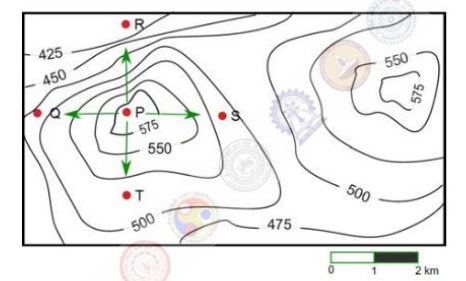
\includegraphics[width=0.5\textwidth]{figures/10.png}
\end{center}

Which of the following is the steepest path leaving from P?}{10}
\begin{enumerate}
    \item[(A)] P to Q
    \item[(B)] P to R
    \item[(C)] P to S
    \item[(D)] P to T
\end{enumerate}

\vspace{0.5cm}

% Technical Section
\section*{Technical Section}

\questiona{The rank of the matrix  
\[\begin{bmatrix}
1 & -1 & 0 & 0 & 0 \\
0 & 0 & 1 & -1 & 0 \\
0 & 1 & -1 & 0 & 0 \\
-1 & 0 & 0 & 0 & 1 \\
0 & 0 & 0 & 1 & -1
\end{bmatrix}\]
is \_\_\_\_\_.}{1}

\vspace{0.5cm}

\questiona{The general solution of the differential equation  
\[\frac{d^2 y}{dx^2} + 2 \frac{dy}{dx} - 5y = 0\]
in terms of arbitrary constants \( K_1 \) and \( K_2 \) is}{2}
\begin{enumerate}
    \item[(A)] \( K_1 e^{\left(-1+\sqrt{6}\right)x} + K_2 e^{\left(-1-\sqrt{6}\right)x} \)
    \item[(B)] \( K_1 e^{\left(-1+\sqrt{8}\right)x} + K_2 e^{\left(-1-\sqrt{8}\right)x} \)
    \item[(C)] \( K_1 e^{\left(-2+\sqrt{6}\right)x} + K_2 e^{\left(-2-\sqrt{6}\right)x} \)
    \item[(D)] \( K_1 e^{\left(-2+\sqrt{8}\right)x} + K_2 e^{\left(-2-\sqrt{8}\right)x} \)
\end{enumerate}

\vspace{0.5cm}

\questiona{The smaller angle (in degrees) between the planes \( x + y + z = 1 \) and \( 2x - y + 2z = 0 \) is \_\_\_\_\_.}{3}

\vspace{0.5cm}

\questiona{The residues of a function  
\[ f(z) = \frac{1}{(z - 4)(z + 1)^3} \]  
are}{4}
\begin{enumerate}
    \item[(A)] \(\frac{-1}{27}\) and \(\frac{-1}{125}\)
    \item[(B)] \(\frac{1}{125}\) and \(\frac{-1}{125}\)
    \item[(C)] \(\frac{-1}{27}\) and \(\frac{1}{5}\)
    \item[(D)] \(\frac{1}{125}\) and \(\frac{-1}{5}\)
\end{enumerate}

\vspace{0.5cm}

\questiona{In the circuit shown, \(V\) is a sinusoidal voltage source. The current \(I\) is in phase with voltage \(V\). The ratio  
\[\frac{\text{amplitude of voltage across the capacitor}}{\text{amplitude of voltage across the resistor}}\]  
is \_\_\_\_\_.}{5}

\begin{center}
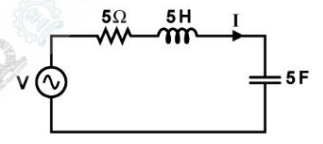
\includegraphics[width=0.5\textwidth]{figures/5.png}
\end{center}

\vspace{0.5cm}

\questiona{A connection is made consisting of resistance \(A\) in series with a parallel combination of resistances \(B\) and \(C\). Three resistors of value \(10\,\Omega\), \(5\,\Omega\), \(2\,\Omega\) are provided. Consider all possible permutations of the given resistors into the positions \(A\), \(B\), \(C\), and identify the configurations with maximum possible overall resistance, and also the ones with minimum possible overall resistance. The ratio of maximum to minimum values of the resistances (up to second decimal place) is \_\_\_\_\_.}{6}

\vspace{0.5cm}

\questiona{An LTI system with unit sample response is a  
\[ h[n] = 5\delta[n] - 7\delta[n-1] + 7\delta[n-3] - 5\delta[n-4] \]  
is a}{7}
\begin{enumerate}
    \item[(A)] low-pass filter
    \item[(B)] high-pass filter
    \item[(C)] band-pass filter
    \item[(D)] band-stop filter
\end{enumerate}

\vspace{0.5cm}

\questiona{The input \( x(t) \) and the output \( y(t) \) of a continuous-time system are related as  
\[ y(t) = \int_{t-T}^t x(u) \, du. \]  
The system is}{8}
\begin{enumerate}
    \item[(A)] linear and time-variant
    \item[(B)] linear and time-invariant
    \item[(C)] non-linear and time-variant
    \item[(D)] non-linear and time-invariant
\end{enumerate}

\vspace{0.5cm}

\questiona{An \( n \)-channel enhancement mode MOSFET is biased at \( V_{GS} > V_{TH} \) and \( V_{DS} > (V_{GS} - V_{TH}) \), where \( V_{GS} \) is the gate-to-source voltage, \( V_{DS} \) is the drain-to-source voltage and \( V_{TH} \) is the threshold voltage. Considering channel length modulation effect to be significant, the MOSFET behaves as a}{9}
\begin{enumerate}
    \item[(A)] voltage source with zero output impedance
    \item[(B)] voltage source with non-zero output impedance
    \item[(C)] current source with finite output impedance
    \item[(D)] current source with infinite output impedance
\end{enumerate}

\vspace{0.5cm}

\questiona{An npn bipolar junction transistor (BJT) is operating in the active region. If the reverse bias across the base-collector junction is increased, then}{10}
\begin{enumerate}
    \item[(A)] the effective base width increases and common-emitter current gain increases
    \item[(B)] the effective base width increases and common-emitter current gain decreases
    \item[(C)] the effective base width decreases and common-emitter current gain increases
    \item[(D)] the effective base width decreases and common-emitter current gain decreases
\end{enumerate}

\vspace{0.5cm}

\questiona{Consider an $n$-channel MOSFET having width $W$, length $L$, electron mobility in the channel $\mu_n$ and oxide capacitance per unit area $C_{ox}$. If gate-to-source voltage $V_{GS} = 0.7\,\text{V}$, drain-to-source voltage $V_{DS} = 0.1\,\text{V}$, $(\mu_n C_{ox}) = 100\,\mu\text{A/V}^2$, threshold voltage $V_{TH} = 0.3\,\text{V}$ and $(W/L) = 50$, then the transconductance $g_m$ (in mA/V) is \_\_\_\_\_.}{11}

\vspace{0.5cm}

\questiona{The output $V_0$ of the diode circuit shown in the figure is connected to an averaging DC voltmeter. The reading on the DC voltmeter in Volts, neglecting the voltage drop across the diode, is \_\_\_\_\_.
\begin{center}
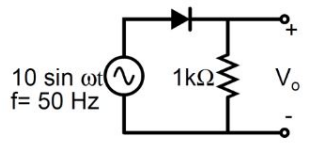
\includegraphics[width=0.5\textwidth]{figures/12.png}
\end{center}}{12}

\vspace{0.5cm}

\questiona{In the figure, D1 is a real silicon $pn$ junction diode with a drop of 0.7 V under forward bias condition and D2 is a Zener diode with breakdown voltage of $-6.8\,\text{V}$. The input $V_{\text{in}}(t)$ is a periodic square wave of period T, whose one period is shown in the figure.
\begin{center}
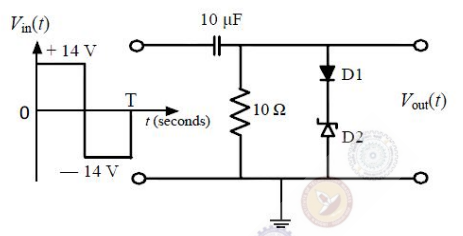
\includegraphics[width=0.5\textwidth]{figures/13.png}
\end{center}
Assuming $10\tau << T$, the maximum and minimum values of the output waveform are respectively}{13}
\begin{enumerate}
    \item[(A)] 7.5 V and $-20.5\,\text{V}$
    \item[(B)] 6.1 V and $-21.9\,\text{V}$
    \item[(C)] 7.5 V and $-21.2\,\text{V}$
    \item[(D)] 6.1 V and $-22.6\,\text{V}$
\end{enumerate}

\vspace{0.5cm}

\questiona{Consider the circuit shown in the figure. Assume base-to-emitter voltage $V_{BE} = 0.8\,\text{V}$ and common-base current gain ($\alpha$) of the transistor is unity.
\begin{center}
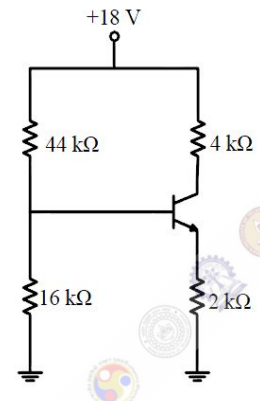
\includegraphics[width=0.5\textwidth]{figures/14.png}
\end{center}
The value of the collector-to-emitter voltage $V_{CE}$ (in volt) is \_\_\_\_\_.}{14}

\vspace{0.5cm}

\questiona{For the circuit shown in the figure, $P$ and $Q$ are the inputs and $Y$ is the output.
\begin{center}
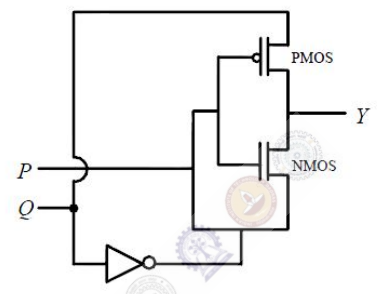
\includegraphics[width=0.5\textwidth]{figures/15.png}
\end{center}
The logic implemented by the circuit is}{15}
\begin{enumerate}
    \item[(A)] XNOR
    \item[(B)] XOR
    \item[(C)] NOR
    \item[(D)] OR
\end{enumerate}

\vspace{0.5cm}

\questiona{Consider the circuit shown in the figure.
\begin{center}
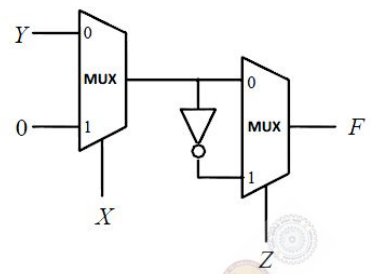
\includegraphics[width=0.5\textwidth]{figures/16.png}
\end{center}
The Boolean expression $F$ implemented by the circuit is}{16}
\begin{enumerate}
    \item[(A)] $\bar{X}\bar{Y}Z + XY + \bar{Y}Z$
    \item[(B)] $\bar{X}YZ + XZ + \bar{Y}Z$
    \item[(C)] $\bar{X}YZ + XY + \bar{Y}Z$
    \item[(D)] $\bar{X}YZ + XZ + \bar{Y}Z$
\end{enumerate}

\vspace{0.5cm}

\questiona{In a DRAM,}{17}
\begin{enumerate}
    \item[(A)] periodic refreshing is not required
    \item[(B)] information is stored in a capacitor
    \item[(C)] information is stored in a latch
    \item[(D)] both read and write operations can be performed simultaneously
\end{enumerate}

\vspace{0.5cm}

\questiona{For the system shown in the figure, $Y(s)/X(s) = $ \_\_\_\_\_.
\begin{center}
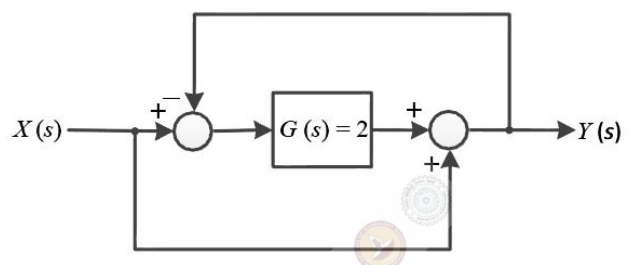
\includegraphics[width=0.5\textwidth]{figures/18.png}
\end{center}}{18}

\vspace{0.5cm}

\questiona{Consider the state space realization
\[
\begin{bmatrix}
\dot{x}_1(t) \\
\dot{x}_2(t)
\end{bmatrix} =
\begin{bmatrix}
0 & 0 \\
0 & -9
\end{bmatrix}
\begin{bmatrix}
x_1(t) \\
x_2(t)
\end{bmatrix}
+
\begin{bmatrix}
0 \\
45
\end{bmatrix}
u(t),
\]
with initial condition $\begin{bmatrix}x_1(0) \\ x_2(0)\end{bmatrix} = \begin{bmatrix}0 \\ 0\end{bmatrix}$,
where $u(t)$ is the unit step function. The value of $\lim\limits_{t\to\infty}\left|\sqrt{x_1^2(t)+x_2^2(t)}\right|$ is \_\_\_\_\_.}{19}

\vspace{0.5cm}

\questiona{Which of the following statements is \textbf{incorrect}?}{20}
\begin{enumerate}
    \item[(A)] Lead compensator is used to reduce the settling time.
    \item[(B)] Lag compensator is used to reduce the steady state error.
    \item[(C)] Lead compensator may increase the order of a system.
    \item[(D)] Lag compensator always stabilizes an unstable system.
\end{enumerate}

\vspace{0.5cm}

\questiona{Which one of the following graphs shows the Shannon capacity (channel capacity) in bits of a memoryless binary symmetric channel with crossover probability $p$?}{21}
\begin{center}
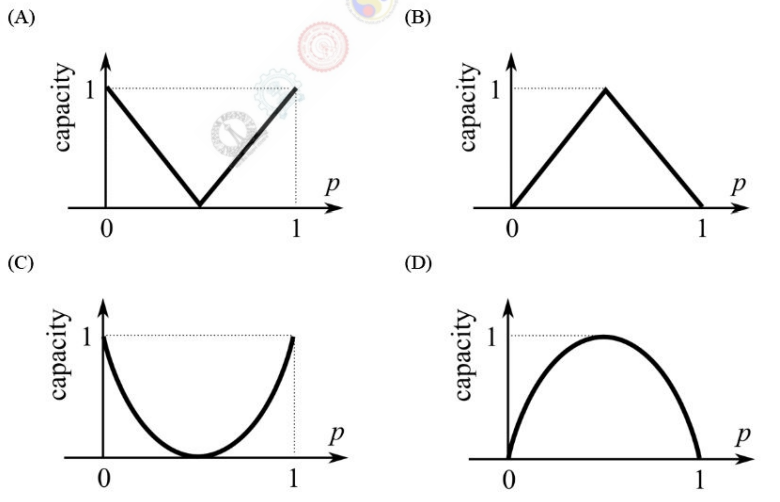
\includegraphics[width=0.9\textwidth]{figures/21.png}
\end{center}

\vspace{0.5cm}

\questiona{Consider the random process $X(t) = U + Vt$, where $U$ is a zero-mean Gaussian random variable and $V$ is uniformly distributed between 0 and 2. The mean value of the random process at $t = 2$ is \_\_\_\_\_.}{22}

\vspace{0.5cm}

\questiona{A sinusoidal message signal is converted to a PCM signal using a uniform quantizer. The required signal-to-quantization noise ratio (SQNR) at the output of the quantizer is 40 dB. The minimum number of bits per sample needed to achieve the desired SQNR is \_\_\_\_\_.}{23}

\vspace{0.5cm}

\questiona{Two conducting spheres S1 and S2 of radii $a$ and $b$ ($b > a$) respectively, are placed far apart and connected by a long, thin conducting wire.
\begin{center}
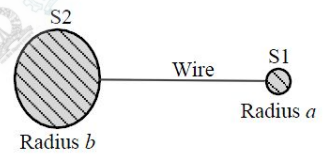
\includegraphics[width=0.5\textwidth]{figures/24.png}
\end{center}

For some charge placed on this structure, the potential and surface electric field on S1 are $V_a$ and $E_a$, and that on S2 are $V_b$ and $E_b$, respectively. Then, which of the following is \textbf{CORRECT}?}{24}
\begin{enumerate}
    \item[(A)] $V_a = V_b$ and $E_a < E_b$
    \item[(B)] $V_a > V_b$ and $E_a > E_b$
    \item[(C)] $V_a = V_b$ and $E_a > E_b$
    \item[(D)] $V_a > V_b$ and $E_a = E_b$
\end{enumerate}

\vspace{0.5cm}

\questiona{A two-wire transmission line terminates in a television set. The VSWR measured on the line is 5.8. The percentage of power that is reflected from the television set is \_\_\_\_\_.}{25}

\vspace{0.5cm}

\questionb{The values of the integrals 
\[
\int_{0}^{1} \left( \int_{0}^{1} \frac{x - y}{(x + y)^3} dy \right) dx
\]
and
\[
\int_{0}^{1} \left( \int_{0}^{1} \frac{x - y}{(x + y)^3} dx \right) dy
\]
are}{26}
\begin{enumerate}
    \item[(A)] same and equal to 0.5
    \item[(B)] same and equal to $-0.5$
    \item[(C)] 0.5 and $-0.5$, respectively
    \item[(D)] $-0.5$ and 0.5, respectively
\end{enumerate}

\vspace{0.5cm}

\questionb{An integral $I$ over a counterclockwise circle $C$ is given by
\[
I = \oint_C \frac{z^2 - 1}{z^2 + 1} e^z dz.
\]
If $C$ is defined as $|z| = 3$, then the value of $I$ is}{27}
\begin{enumerate}
    \item[(A)] $-\pi i \sin(1)$
    \item[(B)] $-2\pi i \sin(1)$
    \item[(C)] $-3\pi i \sin(1)$
    \item[(D)] $-4\pi i \sin(1)$
\end{enumerate}

\vspace{0.5cm}

\questionb{If the vector function $\vec{F} = \vec{a}_x (3y - k_1 z) + \vec{a}_y (k_2 x - 2z) - \vec{a}_z (k_3 y + z)$ is irrotational, then the values of the constants $k_1$, $k_2$ and $k_3$, respectively, are}{28}
\begin{enumerate}
    \item[(A)] 0.3, $-2.5$, 0.5
    \item[(B)] 0.0, 3.0, 2.0
    \item[(C)] 0.3, 0.33, 0.5
    \item[(D)] 4.0, 3.0, 2.0
\end{enumerate}

\vspace{0.5cm}

\questionb{Passengers try repeatedly to get a seat reservation in any train running between two stations until they are successful. If there is 40\% chance of getting reservation in any attempt by a passenger, then the average number of attempts that passengers need to make to get a seat reserved is \_\_\_\_\_.}{29}

\vspace{0.5cm}

\questionb{The minimum value of the function $f(x) = \frac{1}{3}x(x^2 - 3)$ in the interval $-100 \leq x \leq 100$ occurs at $x = $ \_\_\_\_\_.}{30}

\vspace{0.5cm}

\questionb{The switch in the circuit shown in the figure was open for a long time and is closed at $t = 0$.
\begin{center}
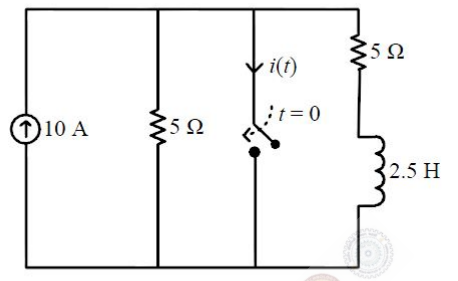
\includegraphics[width=0.5\textwidth]{figures/31.png}
\end{center}
The current $i(t)$ (in ampere) at $t = 0.5$ seconds is \_\_\_\_\_.}{31}

\vspace{0.5cm}

\questionb{Consider the circuit shown in the figure.
\begin{center}
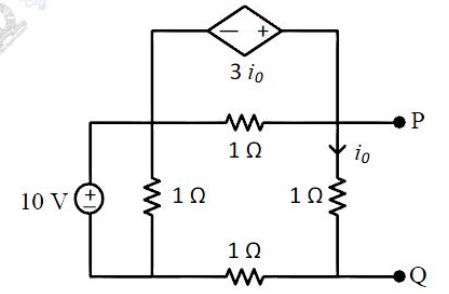
\includegraphics[width=0.5\textwidth]{figures/32.png}
\end{center}
The Thevenin equivalent resistance (in $\Omega$) across P-Q is \_\_\_\_\_.}{32}

\vspace{0.5cm}

\questionb{Consider an LTI system with magnitude response
\[
|H(f)| = 
\begin{cases} 
1 - \frac{|f|}{20}, & |f| \leq 20 \\ 
0, & |f| > 20 
\end{cases}
\]
and phase response $\arg \{ H(f) \} = -2f$. If the input is
\[
x(t) = 8 \cos\left(20\pi t + \frac{\pi}{4}\right) + 16 \sin\left(40\pi t + \frac{\pi}{8}\right) + 24 \cos\left(80\pi t + \frac{\pi}{16}\right),
\]
then the average power of the output signal $y(t)$ is \_\_\_\_\_.}{33}

\vspace{0.5cm}

\questionb{The transfer function of a causal LTI system is $H(s) = 1/s$. If the input is $x(t) = \frac{\sin t}{\pi t} u(t)$, where $u(t)$ is a unit step function, the system output $y(t)$ as $t \to \infty$ is \_\_\_\_\_.}{34}

\vspace{0.5cm}

\questionb{Consider the parallel combination of two LTI systems shown in the figure.
\begin{center}
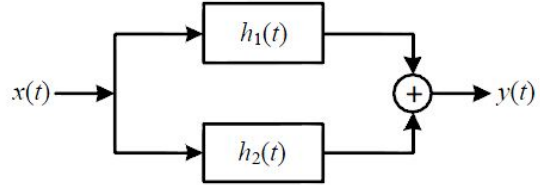
\includegraphics[width=0.5\textwidth]{figures/35.png}
\end{center}
The impulse responses are:
\[
h_1(t) = 2\delta(t+2) - 3\delta(t+1)
\]
\[
h_2(t) = \delta(t-2)
\]
If the input $x(t)$ is a unit step signal, then the energy of $y(t)$ is \_\_\_\_\_.}{35}

\vspace{0.5cm}

\questionb{A MOS capacitor is fabricated on p-type Si (Silicon) where the metal work function is 4.1 eV and electron affinity of Si is 4.0 eV. $E_C - E_F = 0.9$ eV, where $E_C$ and $E_F$ are the conduction band minimum and the Fermi energy levels of Si, respectively. Oxide $\epsilon_r = 3.9$, $\epsilon_o = 8.85 \times 10^{-14}$ F/cm, oxide thickness $t_{ox} = 0.1$ $\mu$m and electronic charge $q = 1.6 \times 10^{-19}$ C. If the measured flat band voltage of this capacitor is $-1$ V, then the magnitude of the fixed charge at the oxide-semiconductor interface, in nC/cm$^2$, is \_\_\_\_\_.}{36}

\vspace{0.5cm}

\questionb{For a particular intensity of incident light on a silicon $pn$ junction solar cell, the photocurrent density ($J_L$) is 2.5 mA/cm$^2$ and the open-circuit voltage ($V_{oc}$) is 0.451 V. Consider thermal voltage ($V_T$) to be 25 mV. If the intensity of the incident light is increased by 20 times, assuming that the temperature remains unchanged, $V_{oc}$ (in volts) will be \_\_\_\_\_.}{37}

\vspace{0.5cm}

\questionb{Two $n$-channel MOSFETs, T1 and T2, are identical in all respects except that the width of T2 is double that of T1. Both transistors are biased in the saturation region of operation, but the gate overdrive voltage ($V_{GS} - V_{TH}$) of T2 is double that of T1, where $V_{GS}$ and $V_{TH}$ are the gate-to-source voltage and threshold voltage of the transistors, respectively. If the drain current and transconductance of T1 are $I_{D1}$ and $g_{m1}$ respectively, the corresponding values for T2 are}{38}
\begin{enumerate}
    \item[(A)] $8I_{D1}$ and $2g_{m1}$
    \item[(B)] $8I_{D1}$ and $4g_{m1}$
    \item[(C)] $4I_{D1}$ and $4g_{m1}$
    \item[(D)] $4I_{D1}$ and $2g_{m1}$
\end{enumerate}

\vspace{0.5cm}

\questionb{An abrupt $pn$ junction (located at $x = 0$) is uniformly doped on both $p$ and $n$ sides. The width of the depletion region is $W$ and the electric field variation in the $x$-direction is $E(x)$. Which of the following figures represents the electric field profile near the $pn$ junction?}{39}
\begin{center}
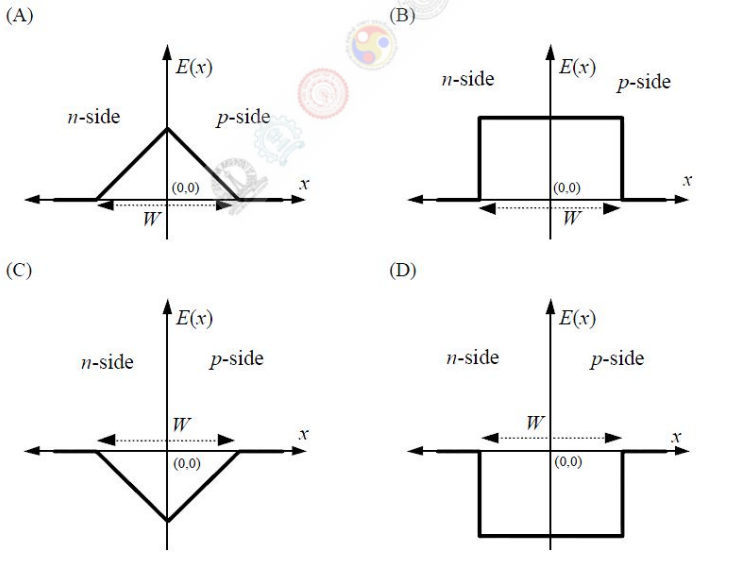
\includegraphics[width=0.9\textwidth]{figures/39.png}
\end{center}

\vspace{0.5cm}

\questionb{Assuming that transistors $M_1$ and $M_2$ are identical and have a threshold voltage of 1 V, the state of transistors $M_1$ and $M_2$ are respectively
\begin{center}
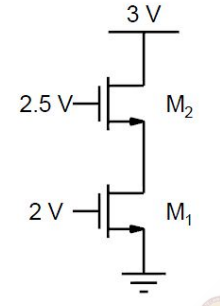
\includegraphics[width=0.4\textwidth]{figures/40.png}
\end{center}}{40}
\begin{enumerate}
    \item[(A)] Saturation, Saturation
    \item[(B)] Linear, Linear
    \item[(C)] Linear, Saturation
    \item[(D)] Saturation, Linear
\end{enumerate}

\vspace{0.5cm}

\questionb{In the circuit shown, transistors $Q_1$ and $Q_2$ are biased at a collector current of 2.6 mA. Assuming transistor current gains are sufficiently large to assume collector current equal to emitter current and thermal voltage of 26 mV, the magnitude of voltage gain $V_o/V_s$ in the mid-band frequency range is \_\_\_\_\_ (up to second decimal place).
\begin{center}
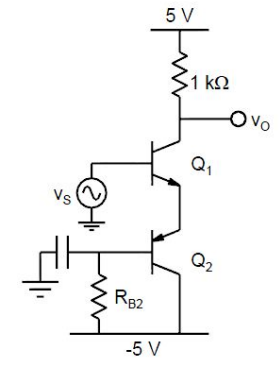
\includegraphics[width=0.5\textwidth]{figures/41.png}
\end{center}}{41}

\vspace{0.5cm}

\questionb{In the voltage reference circuit shown, the op-amp is ideal and transistors $Q_1$, $Q_2$, ..., $Q_{32}$ are identical in all respects and have infinitely large values of common-emitter current gain ($\beta$). The collector current ($I_C$) of the transistors is related to their base-emitter voltage  ($V_B$$_E$) by the relation $I_C = I_S$ exp ($V_B$$_E$/$V_T$), where $I_S$ is the saturation current. Assume that the voltage $V_P$ shown in the figure is 0.7 V and the thermal voltage $V_T$=26 mV.
\begin{center}
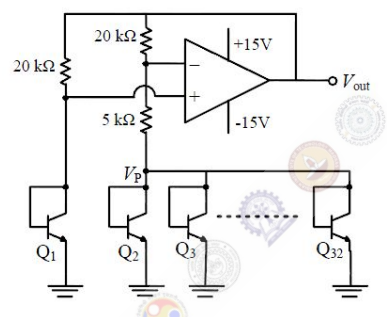
\includegraphics[width=0.5\textwidth]{figures/42.png}
\end{center}
The output voltage $V_{\text{out}}$ (in volts) is \_\_\_\_\_\_\_\_.}{42}

\vspace{0.5cm}

\questionb{The state diagram of a finite state machine (FSM) designed to detect an overlapping sequence of three bits is shown in the figure. The FSM has an input 'In' and an output 'Out'. The initial state of the FSM is $S_0$.
\begin{center}
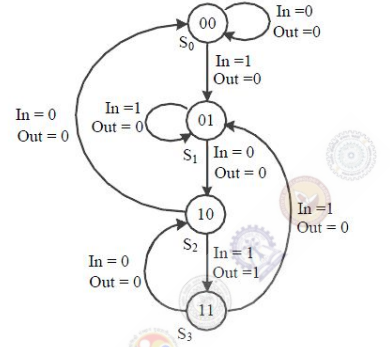
\includegraphics[width=0.5\textwidth]{figures/43.png}
\end{center}
If the input sequence is 10101101001101, starting with the left-most bit, then the number of times 'Out' will be 1 is \_\_\_\_\_\_\_}{43}

\vspace{0.5cm}

\questionb{Figure I shows a 4-bit ripple carry adder realized using full adders and Figure II shows the circuit of a full-adder (FA). The propagation delay of the XOR, AND and OR gates in Figure II are 20 ns, 15 ns and 10 ns, respectively. Assume all the inputs to the 4-bit adder are initially reset to 0.

\begin{center}
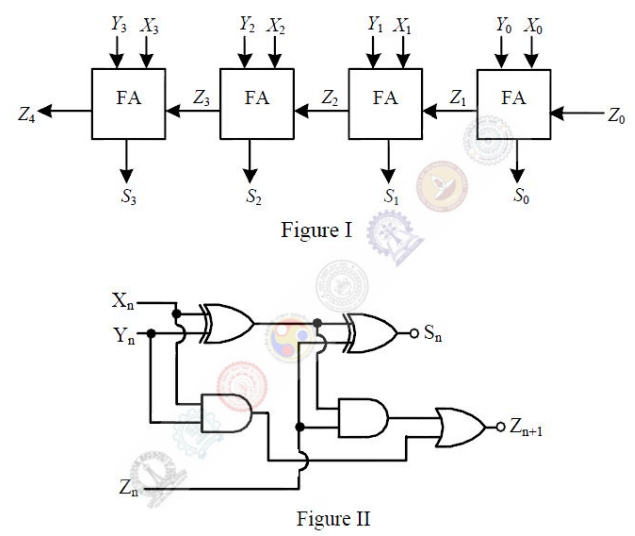
\includegraphics[width=0.7\textwidth]{figures/44.png}
\end{center}

At $t = 0$, the inputs to the 4-bit adder are changed to $X_3X_2X_1X_0 = 1100$, $Y_3Y_2Y_1Y_0 = 0100$ and $Z_0 = 1$. The output of the ripple carry adder will be stable at $t = $ \_\_\_\_\_ ns.}{44}

\vspace{0.5cm}

\questionb{A programmable logic array (PLA) is shown:
\begin{center}
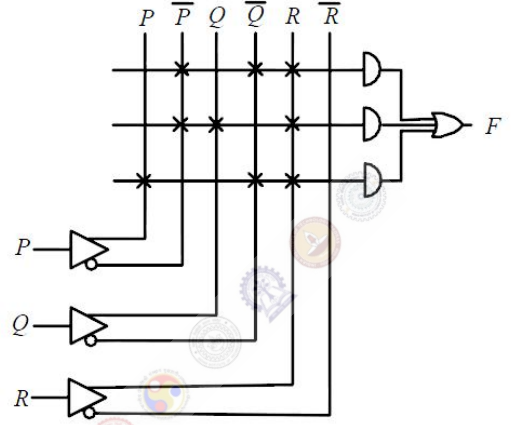
\includegraphics[width=0.5\textwidth]{figures/45.png}
\end{center}
The Boolean function $F$ implemented is}{45}
\begin{enumerate}
    \item[(A)] $\bar{P}\bar{Q}R + \bar{P}QR + P\bar{Q}\bar{R}$
    \item[(B)] $(\bar{P}+\bar{Q}+R)(\bar{P}+Q+R)(P+\bar{Q}+\bar{R})$
    \item[(C)] $\bar{P}\bar{Q}R + \bar{P}QR + P\bar{Q}R$
    \item[(D)] $(\bar{P}+\bar{Q}+R)(\bar{P}+Q+R)(P+\bar{Q}+R)$
\end{enumerate}

\vspace{0.5cm}

\questionb{A unity feedback control system has open-loop transfer function:
\[ G(s) = \frac{2(s+1)}{s^3 + ks^2 + 2s + 1} \]
The value of $k$ for which the system oscillates at 2 rad/s is \_\_\_\_\_.}{46}

\vspace{0.5cm}

\questionb{A second-order LTI system is described by the state equations:
\[
\frac{d}{dt}x_1(t) - x_2(t) = 0
\]
\[
\frac{d}{dt}x_2(t) + 2x_1(t) + 3x_2(t) = r(t)
\]
where $x_1(t)$ and $x_2(t)$ are state variables and $r(t)$ is the input. The output $c(t) = x_1(t)$. The system is}{47}
\begin{enumerate}
    \item[(A)] undamped (oscillatory)
    \item[(B)] underdamped
    \item[(C)] critically damped
    \item[(D)] overdamped
\end{enumerate}

\vspace{0.5cm}

\questionb{A unity feedback control system has open-loop transfer function:
\[
G(s) = \frac{10K(s+2)}{s^3 + 3s^2 + 10}
\]
The Nyquist plot is shown below:
\begin{center}
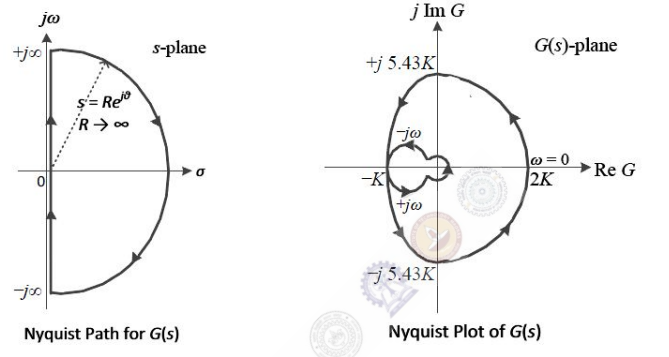
\includegraphics[width=0.8\textwidth]{figures/48.png}
\end{center}
For $0 < K < 1$, the number of closed-loop poles in the right-half s-plane is}{48}
\begin{enumerate}
    \item[(A)] 0
    \item[(B)] 1
    \item[(C)] 2
    \item[(D)] 3
\end{enumerate}

\vspace{0.5cm}

\questionb{The signal \( x(t) = \sin(14000\pi t) \), where \( t \) is in seconds, is sampled at a rate of 9000 samples per second. The sampled signal is the input to an ideal lowpass filter with frequency response \( H(f) \) as follows:

\[
H(f) = 
\begin{cases} 
1, & |f| \leq 12 \text{ kHz} \\
0, & |f| > 12 \text{ kHz} .
\end{cases}
\]

What is the number of sinusoids in the output and their frequencies in kHz?}{49}
\begin{enumerate}
    \item[(A)] Number = 1, frequency = 7
    \item[(B)] Number = 3, frequencies = 2,7,11
    \item[(C)] Number = 2, frequencies = 2,7
    \item[(D)] Number = 2, frequencies = 7,11
\end{enumerate}

\vspace{0.5cm}

\questionb{The unmodulated carrier power in an AM transmitter is 5 kW. This carrier is modulated by a sinusoidal modulating signal. The maximum percentage of modulation is 50\%. If it is reduced to 40\%, then the maximum unmodulated carrier power (in kW) that can be used without overloading the transmitter is \_\_\_\_\_\_\_\_.}{50}

\vspace{0.5cm}

\questionb{A modulating signal given by $x(t) = 5\sin(4\pi 10^{3}t - 10\pi\cos 2\pi 10^{3}t)$ V is fed to a phase modulator with phase deviation constant $k_p = 5$ rad/V. If the carrier frequency is 20 kHz, the instantaneous frequency (in kHz) at $t = 0.5$ ms is \_\_\_\_\_.}{51}

\vspace{0.5cm}

\questionb{Consider a binary memoryless channel characterized by the transition probability diagram:
\begin{center}
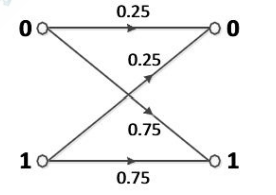
\includegraphics[width=0.4\textwidth]{figures/52.png}
\end{center}
The channel is}{52}
\begin{enumerate}
    \item[(A)] lossless
    \item[(B)] noiseless
    \item[(C)] useless
    \item[(D)] deterministic
\end{enumerate}

\vspace{0.5cm}

\questionb{An electron ($q_1$) is moving in free space with velocity $10^5$ m/s towards a stationary ($q_2$) far away. The closest distance that this moving electron gets to the stationary electron before the repulsive force diverts its path is \_\_\_\_\_ $\times 10^{-8}$ F/m. 
[Given: $m_e = 9.11 \times 10^{-31}$ kg, $e = -1.6 \times 10^{-19}$ C, $\varepsilon_0 = \frac{10^{-9}}{36\pi}$ F/m]}{53}

\vspace{0.5cm}

\questionb{Standard air-filled rectangular waveguides of dimensions $a = 2.29$ cm and $b = 1.02$ cm are designed for radar applications. It is desired that these waveguides operate only in the dominant TE$_{10}$ mode with the operating frequency at least 25\% above the cutoff frequency of the TE$_{10}$ mode but not higher than 95\% of the next higher cutoff frequency. The range of the allowable operating frequency $f$ is}{54}
\begin{enumerate}
    \item[(A)] $8.19$ GHz $\leq f \leq 13.1$ GHz
    \item[(B)] $8.19$ GHz $\leq f \leq 12.45$ GHz
    \item[(C)] $6.55$ GHz $\leq f \leq 13.1$ GHz
    \item[(D)] $1.64$ GHz $\leq f \leq 10.24$ GHz
\end{enumerate}

\vspace{0.5cm}

\questionb{The permittivity of water at optical frequencies is 1.75 $\varepsilon_0$. It is found that an isotropic light source at a distance d under water forms an illuminated circular area of radius 5 m, as shown in the figure. The critical angle is $\theta_C$.
\begin{center}
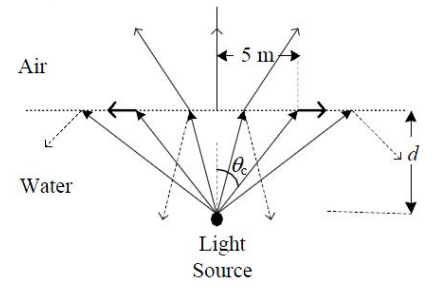
\includegraphics[width=0.5\textwidth]{figures/55.png}
\end{center}
The value of d (in meter) is \_\_\_\_\_\_\_.}{55}

\vspace{5cm}
\begin{center}
\textbf{END OF THE QUESTION PAPER}
\rule{\textwidth}{0.5pt} 
\end{center}

\end{document}
